\subsection{Task 2 Results}
\label{sec:task2results}
\subsubsection{Geometry and Mesh}
As far as grid convergence goes, the same setup, mesh size and material properties, along with adapted boundary conditions have been used in this section. As before, it largest element size was no greater than $3x10^{-3}$m. Many different standalone systems were created inside ANSYS Project Schematic by duplicating the geometries and modifying them to agree with the new Reynolds number and different $L$ values. A sample sketch of the valvular conduit with $L=400$mm and $Re=181$ is shown in Figure \ref{fig:examplesketch} below.\\

\begin{figure}[H]
    \centering
    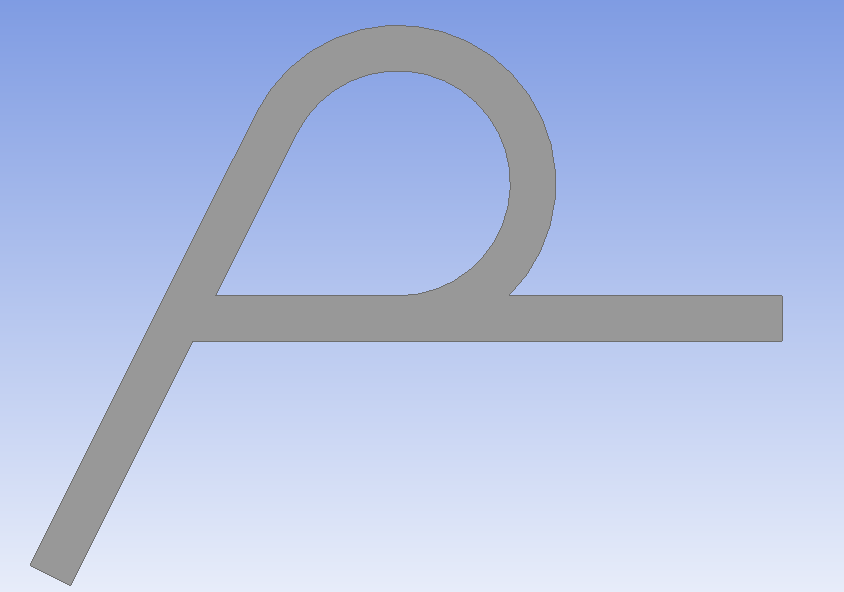
\includegraphics[width = .8\textwidth]{images/task2/sketch_examples/re181.png}
    \caption{Sketch for Re=181 and L=400mm}
    \label{fig:examplesketch}
\end{figure}

\subsubsection{Diodicity Calculations}
The dimensions of the geometry has been modified in each step in accordance with the corresponding Reynolds Numbers and pressure drops in each step have been calculated which is then plugged in to the diodicity formula. The corresponding diodicities are shown on Table \ref{tab:diodicities} below. These results will then be plotted and a curve will be fitted to extract the optimum values.




\begin{table}[H]
\centering
\caption{Diodicities of all configurations}
\label{tab:diodicities}
\resizebox{.4\textwidth}{!}{%
\begin{tabular}{c|ccc}
\hline
\multirow{2}{*}{Re} & \multicolumn{3}{c}{L (mm)}                                      \\ \cline{2-4} 
                    & \multicolumn{1}{c|}{200}   & \multicolumn{1}{c|}{400}   & 600   \\ \hline
181                 & \multicolumn{1}{c|}{1.295} & \multicolumn{1}{c|}{1.200} & 1.131 \\ \hline
362                 & \multicolumn{1}{c|}{1.635} & \multicolumn{1}{c|}{1.705} & 1.471 \\ \hline
543                 & \multicolumn{1}{c|}{1.813} & \multicolumn{1}{c|}{2.434} & 2.244 \\ \hline
\end{tabular}%
}
\end{table}





As can be seen from Figures \ref{fig:l200}, \ref{fig:l400} and \ref{fig:l600} below, pressure values change significantly between the forward and reverse flow cases. Using these plots and the probe method from ANSYS, the pressure drops were calculated. 


%%%%%%%%%%%%%%% L = 200 %%%%%%%%%%%%%
\begin{figure}[H]
 \centering
\begin{subfigure}{.45\textwidth}
  \centering
  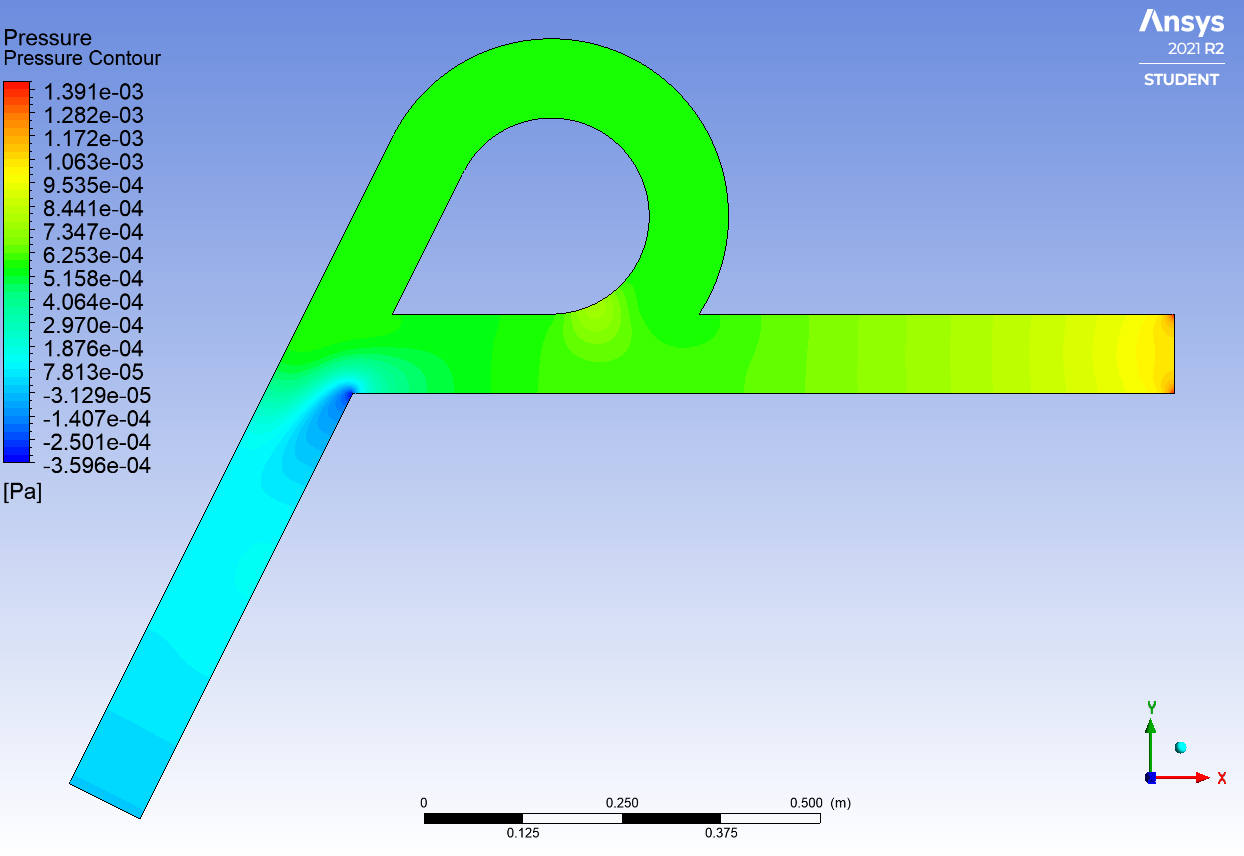
\includegraphics[width=.9\linewidth]{images/task2/L200/forward181.png}
  \caption{Forward flow Re = 181}
  \label{fig:x_d_norm}
\end{subfigure}%
~
\begin{subfigure}{.45\textwidth}
  \centering
  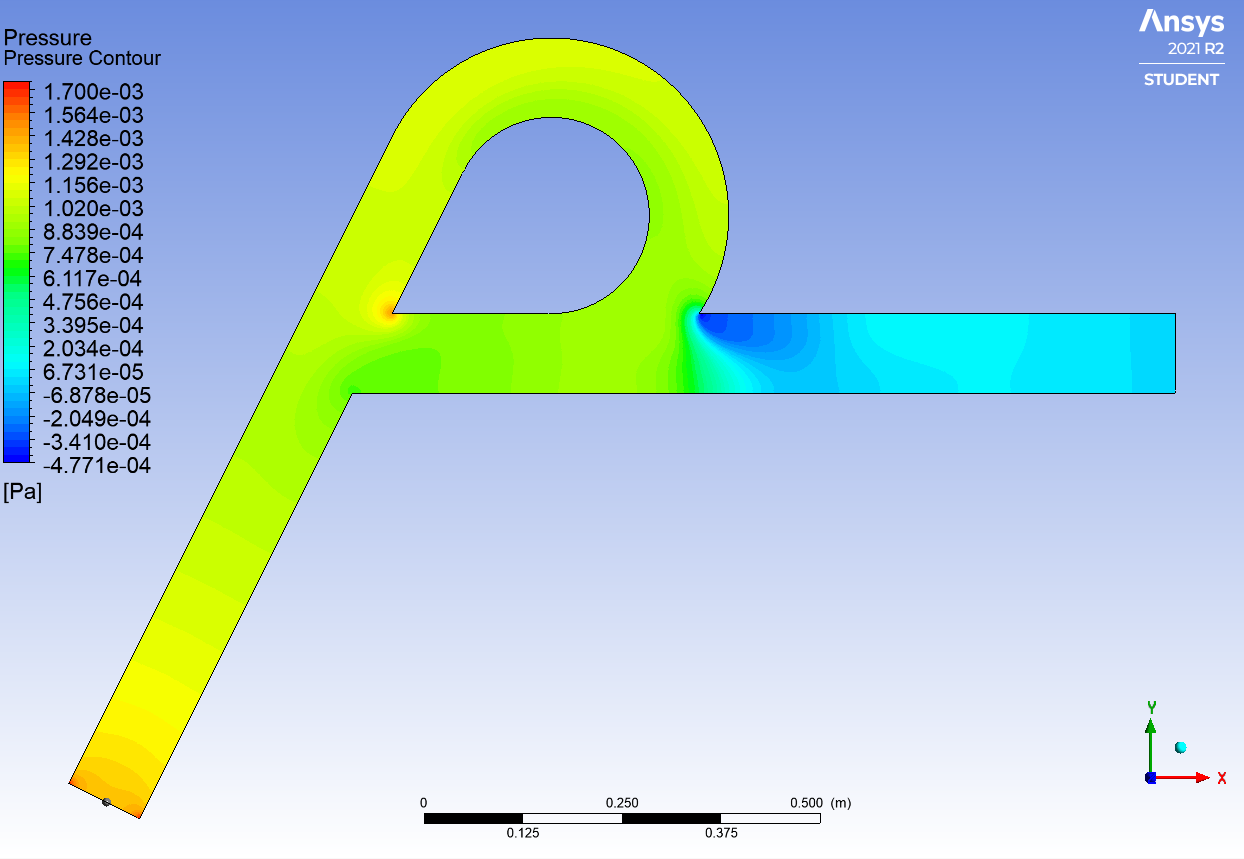
\includegraphics[width=.9\linewidth]{images/task2/L200/reverse181.png}
  \caption{Reverse flow with Re = 181}
  \label{fig:x_d_norm_actual}
\end{subfigure}
~
\begin{subfigure}{.45\textwidth}
  \centering
  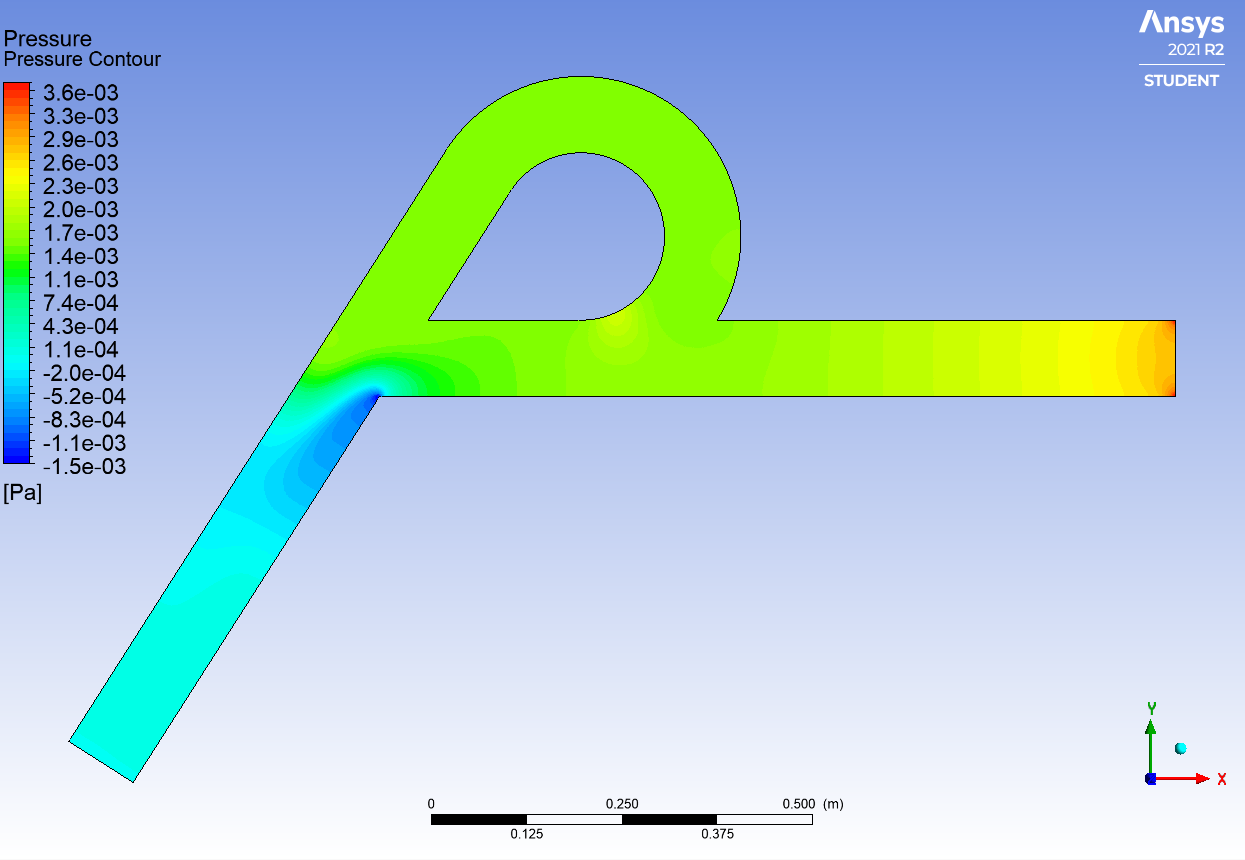
\includegraphics[width=.9\linewidth]{images/task2/L200/forward362.png}
  \caption{Forward flow Re = 362}
  \label{fig:x_d_norm}
\end{subfigure}%
~
\begin{subfigure}{.45\textwidth}
  \centering
  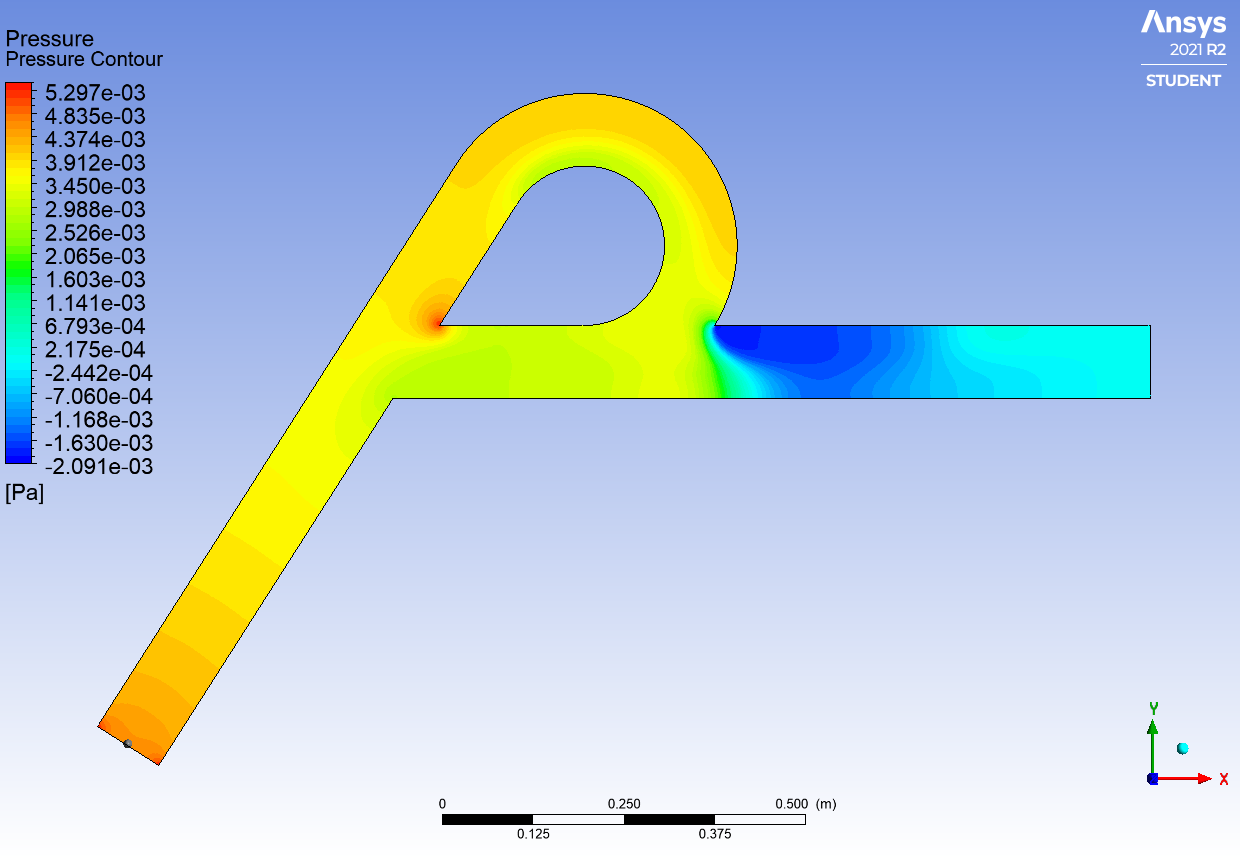
\includegraphics[width=.9\linewidth]{images/task2/L200/reverse362.png}
  \caption{Reverse flow with Re = 362}
  \label{fig:x_d_norm_actual}
\end{subfigure}
~
\begin{subfigure}{.45\textwidth}
  \centering
  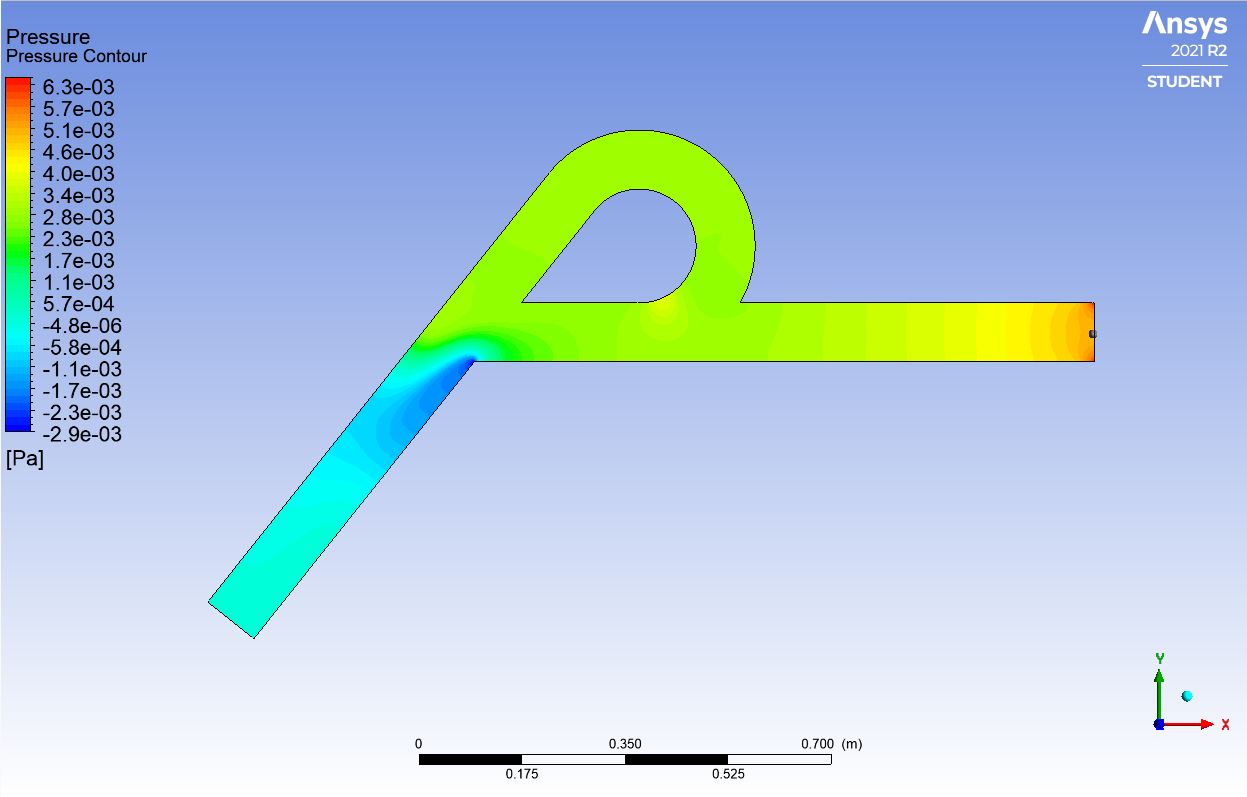
\includegraphics[width=.9\linewidth]{images/task2/L200/forward543.png}
  \caption{Forward flow Re = 543}
  \label{fig:x_d_norm}
\end{subfigure}%
~
\begin{subfigure}{.45\textwidth}
  \centering
  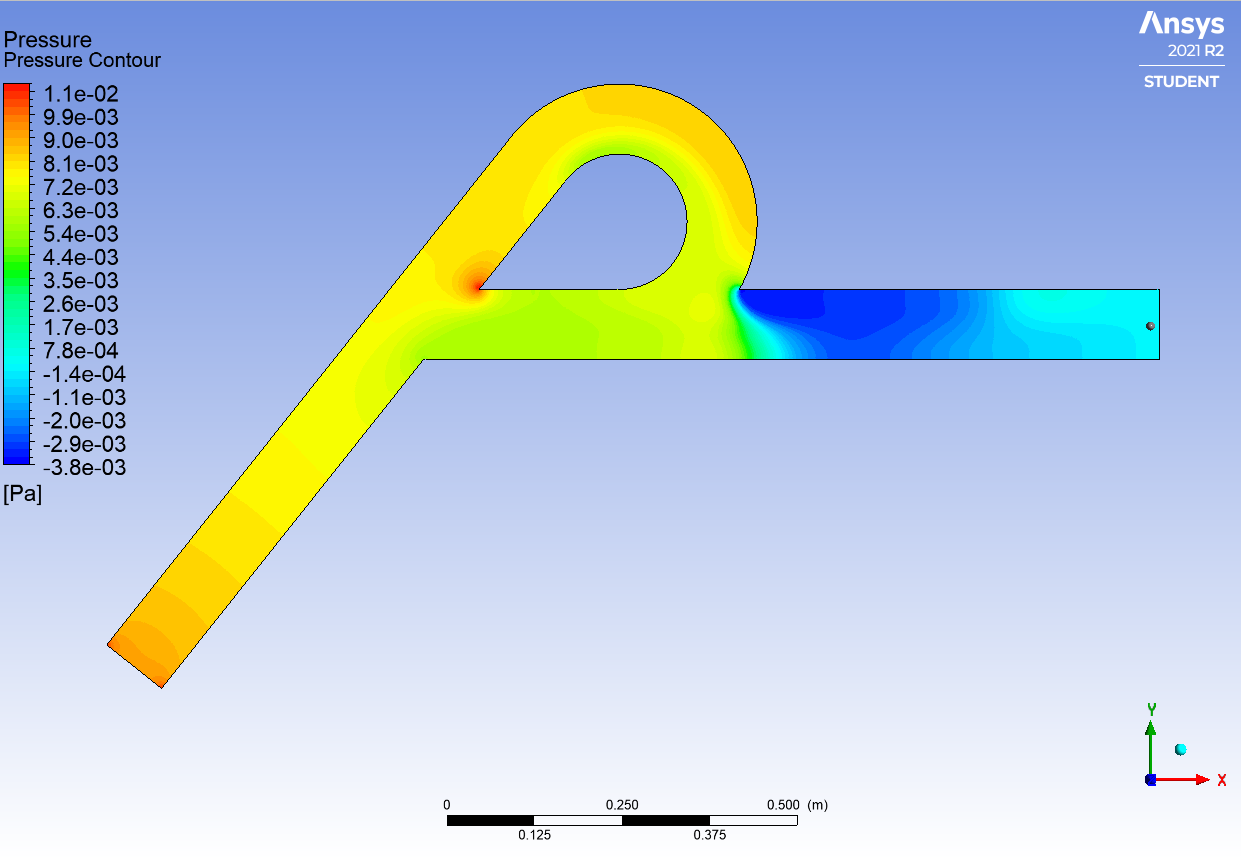
\includegraphics[width=.9\linewidth]{images/task2/L200/reverse543.png}
  \caption{Reverse flow with Re = 543}
  \label{fig:x_d_norm_actual}
\end{subfigure}

\caption{Different Pressure Plots where L = 200mm}
\label{fig:l200}
\end{figure}





%%%%%%%%%% L = 400 %%%%%%%%%%%%%%%%
\begin{figure}[H]
 \centering
\begin{subfigure}{.45\textwidth}
  \centering
  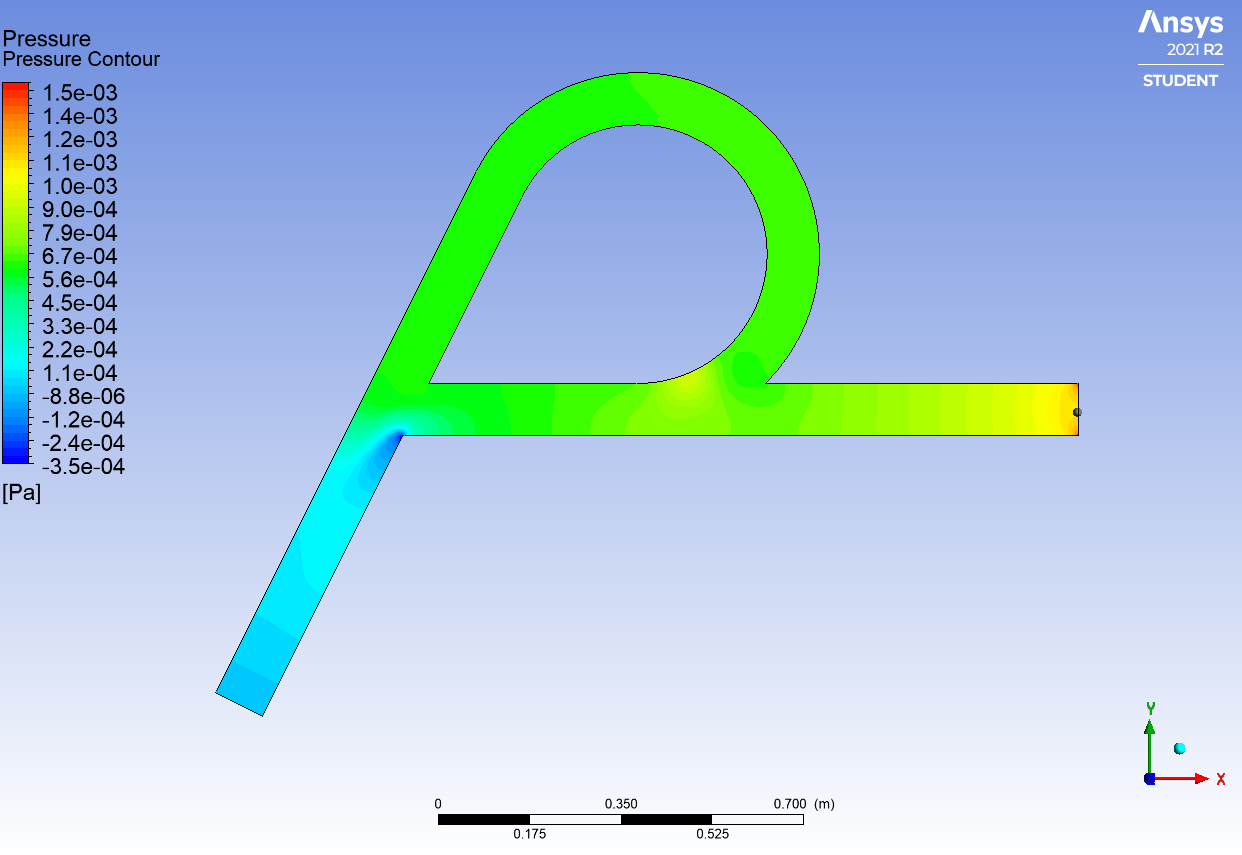
\includegraphics[width=.9\linewidth]{images/task2/L400/forward181.png}
  \caption{Forward flow Re = 181}
  \label{fig:x_d_norm}
\end{subfigure}%
~
\begin{subfigure}{.45\textwidth}
  \centering
  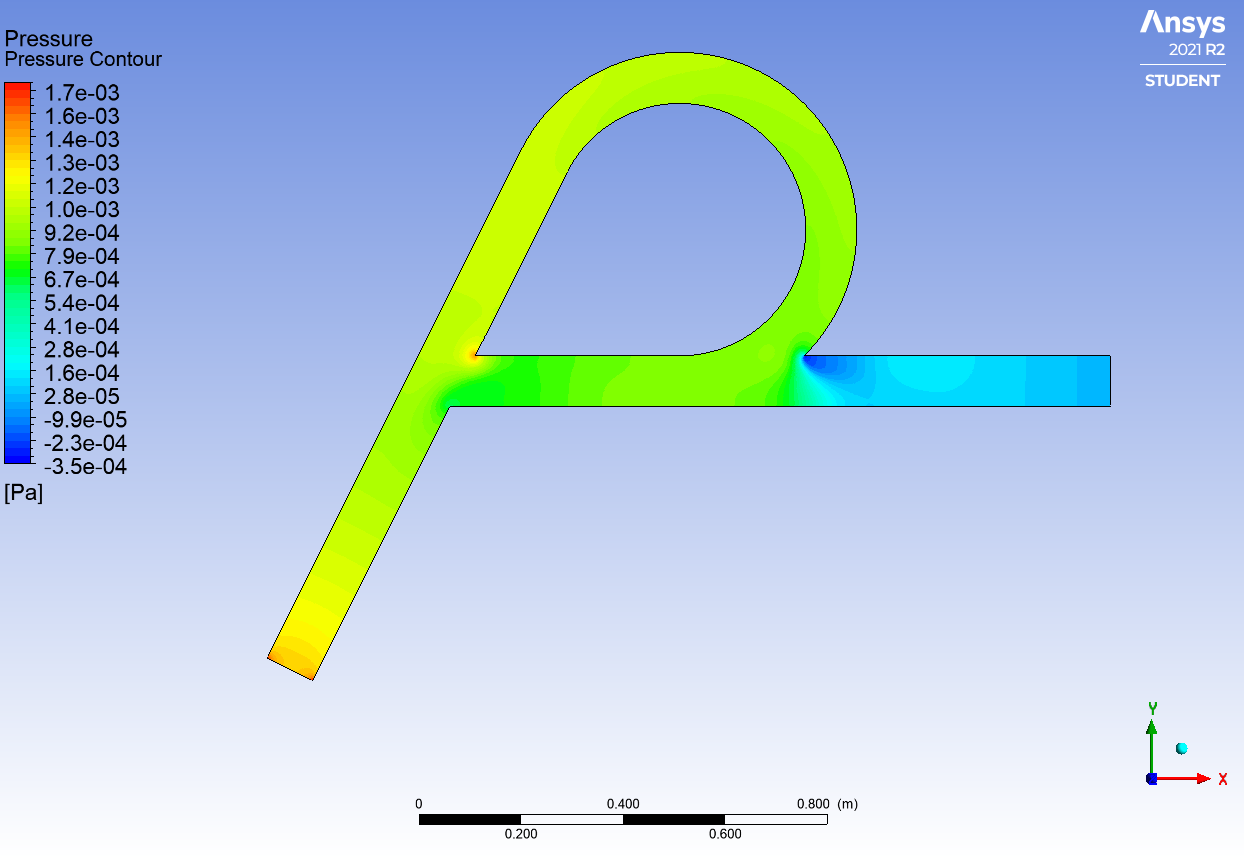
\includegraphics[width=.9\linewidth]{images/task2/L400/reverse181.png}
  \caption{Reverse flow with Re = 181}
  \label{fig:x_d_norm_actual}
\end{subfigure}
~
\begin{subfigure}{.45\textwidth}
  \centering
  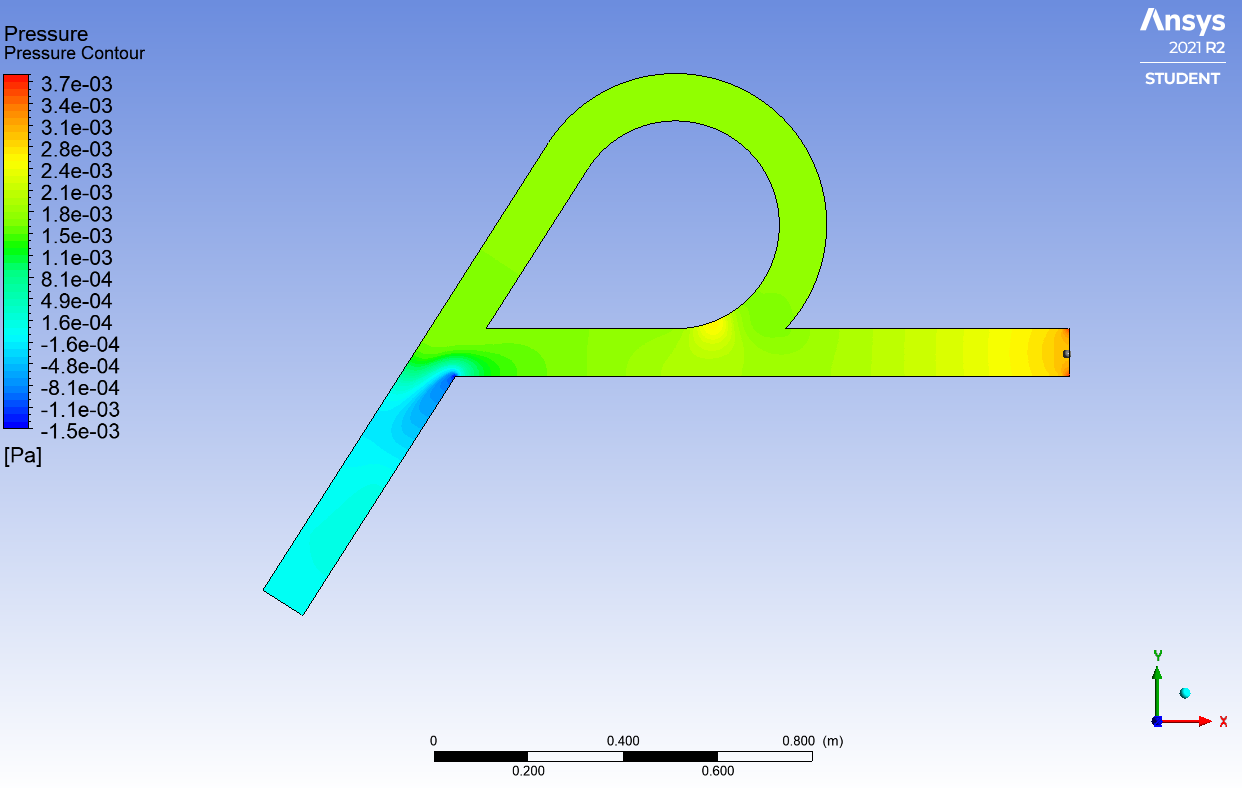
\includegraphics[width=.9\linewidth]{images/task2/L400/forward362.png}
  \caption{Forward flow Re = 362}
  \label{fig:x_d_norm}
\end{subfigure}%
~
\begin{subfigure}{.45\textwidth}
  \centering
  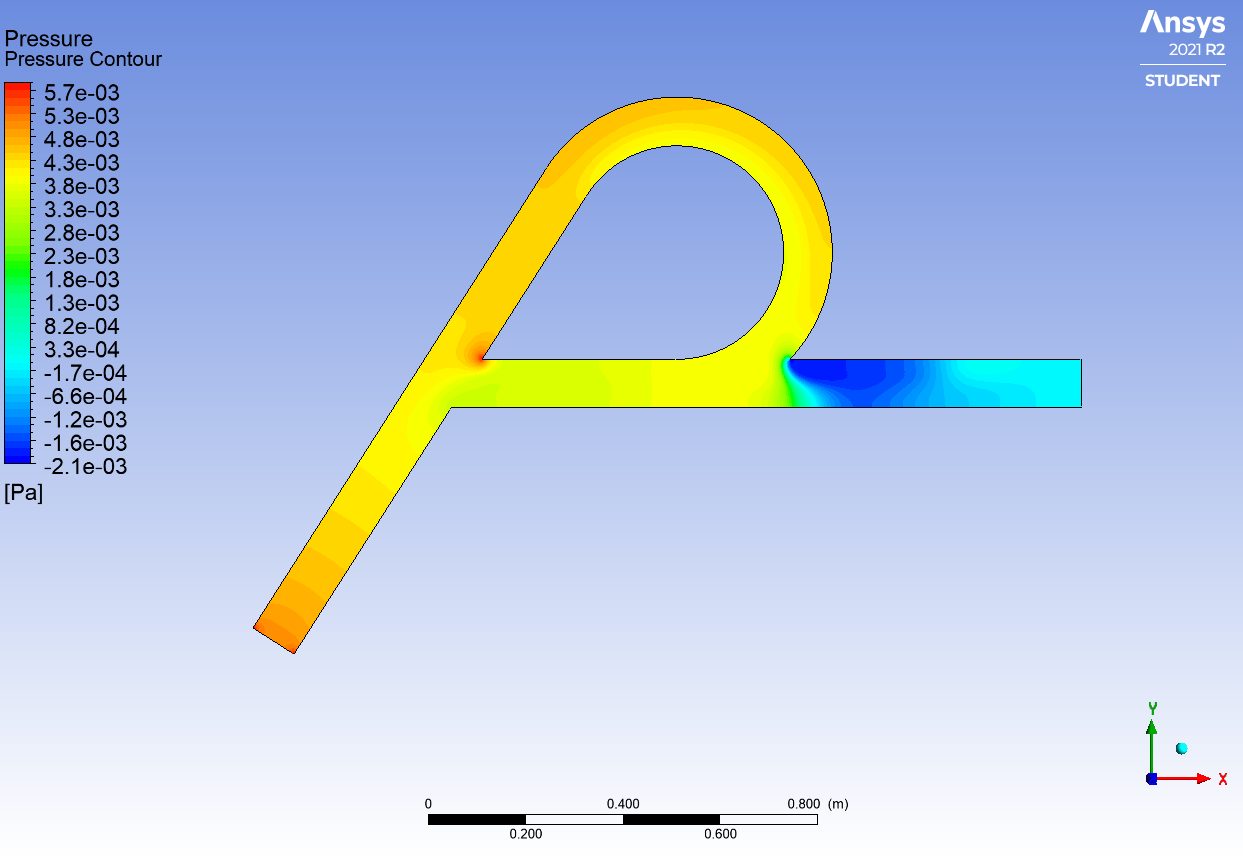
\includegraphics[width=.9\linewidth]{images/task2/L400/reverse362.png}
  \caption{Reverse flow with Re = 362}
  \label{fig:x_d_norm_actual}
\end{subfigure}
~
\begin{subfigure}{.45\textwidth}
  \centering
  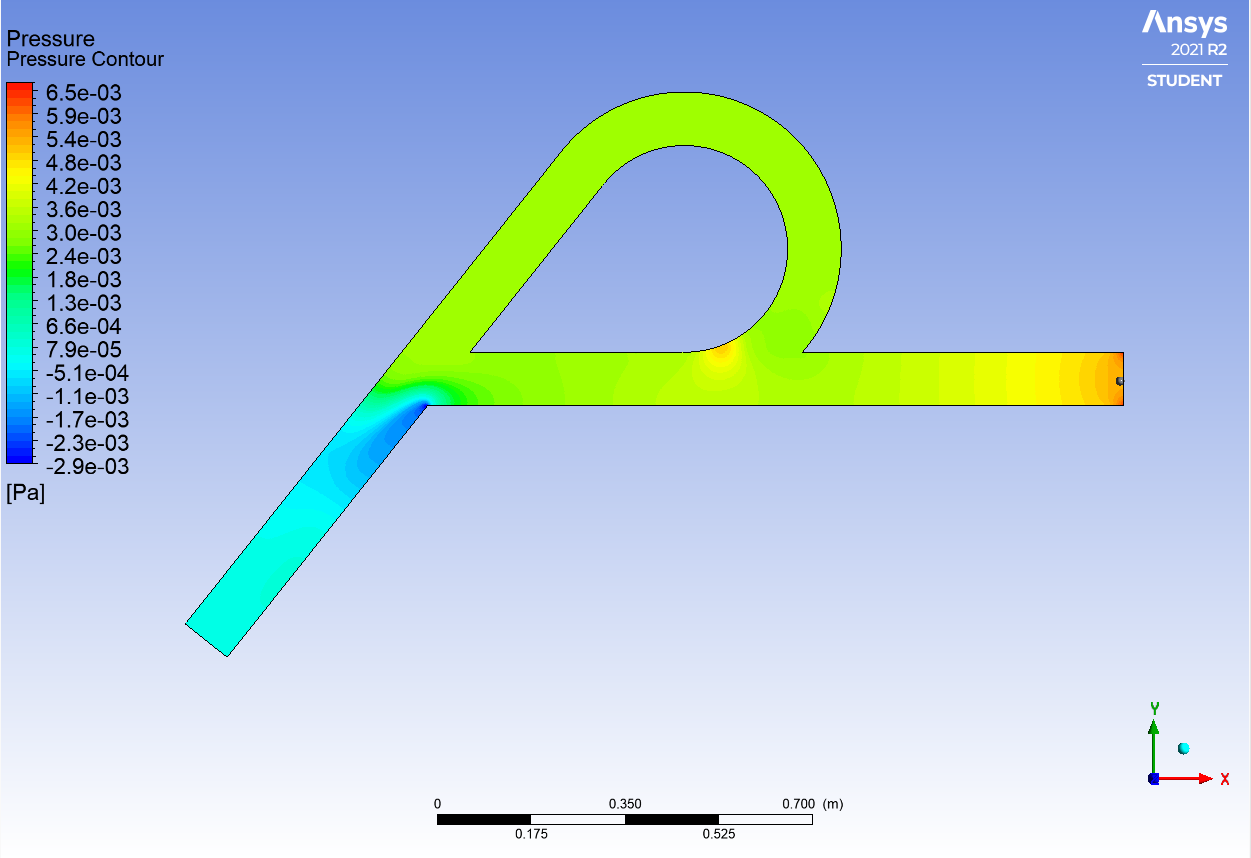
\includegraphics[width=.9\linewidth]{images/task2/L400/forward543.png}
  \caption{Forward flow Re = 543}
  \label{fig:x_d_norm}
\end{subfigure}%
~
\begin{subfigure}{.45\textwidth}
  \centering
  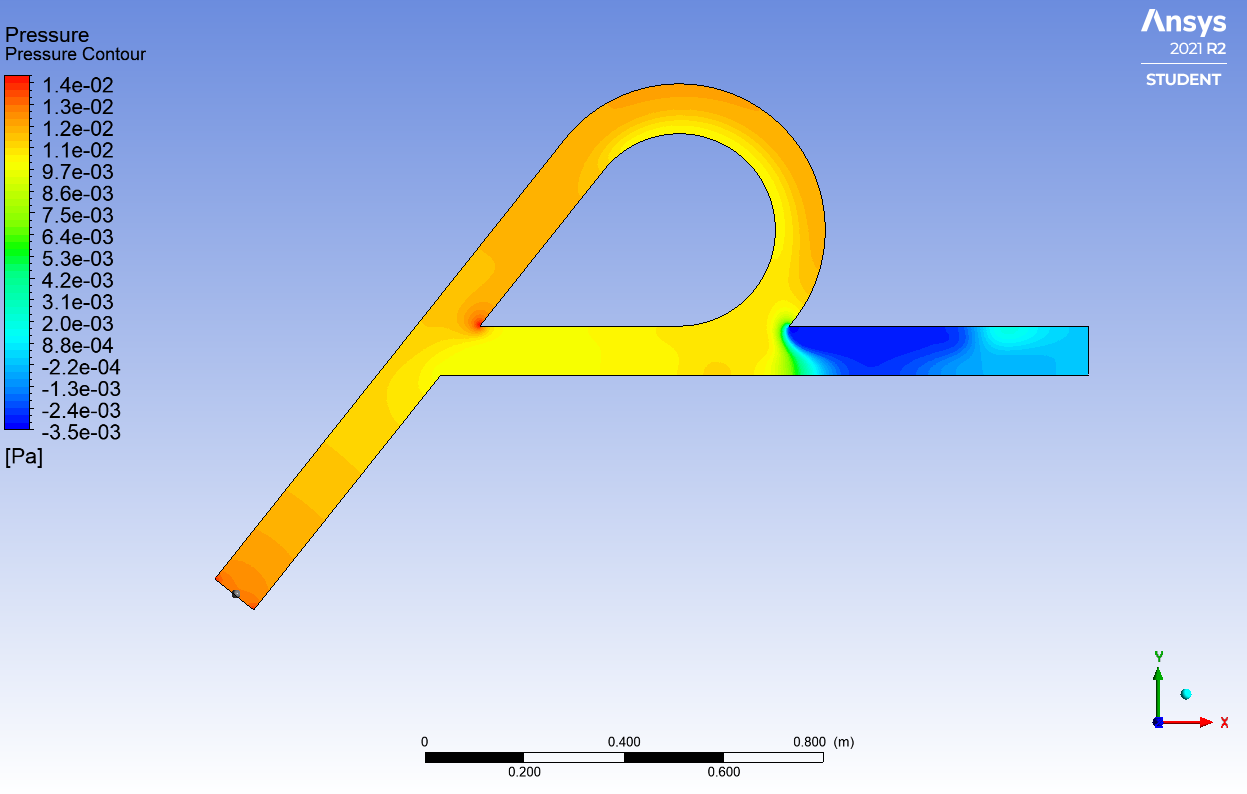
\includegraphics[width=.9\linewidth]{images/task2/L400/reverse543.png}
  \caption{Reverse flow with Re = 543}
  \label{fig:x_d_norm_actual}
\end{subfigure}

\caption{Different Pressure Plots where L = 400mm}
\label{fig:l400}
\end{figure}


%%%%%%%%%% L = 600 %%%%%%%%%%%%%%%%
\begin{figure}[H]
 \centering
\begin{subfigure}{.45\textwidth}
  \centering
  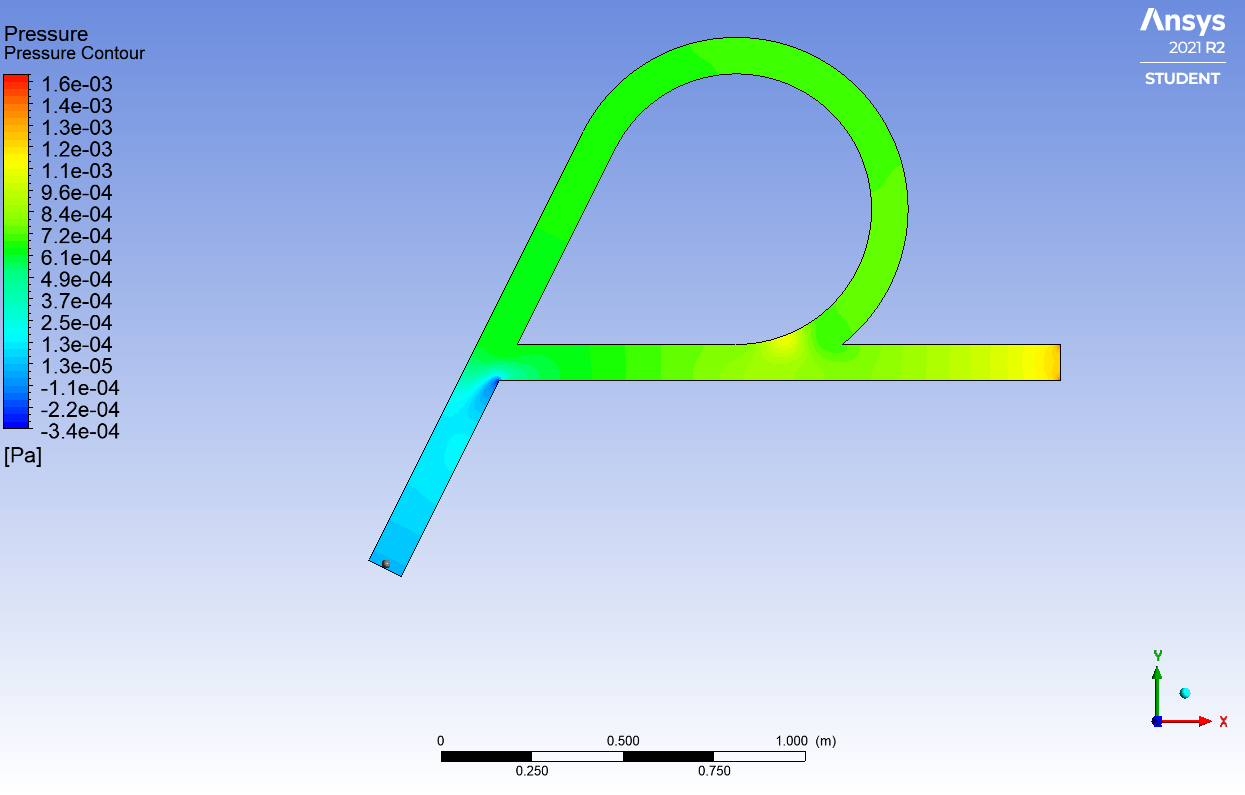
\includegraphics[width=.9\linewidth]{images/task2/L600/forward181.png}
  \caption{Forward flow Re = 181}
  \label{fig:x_d_norm}
\end{subfigure}%
~
\begin{subfigure}{.45\textwidth}
  \centering
  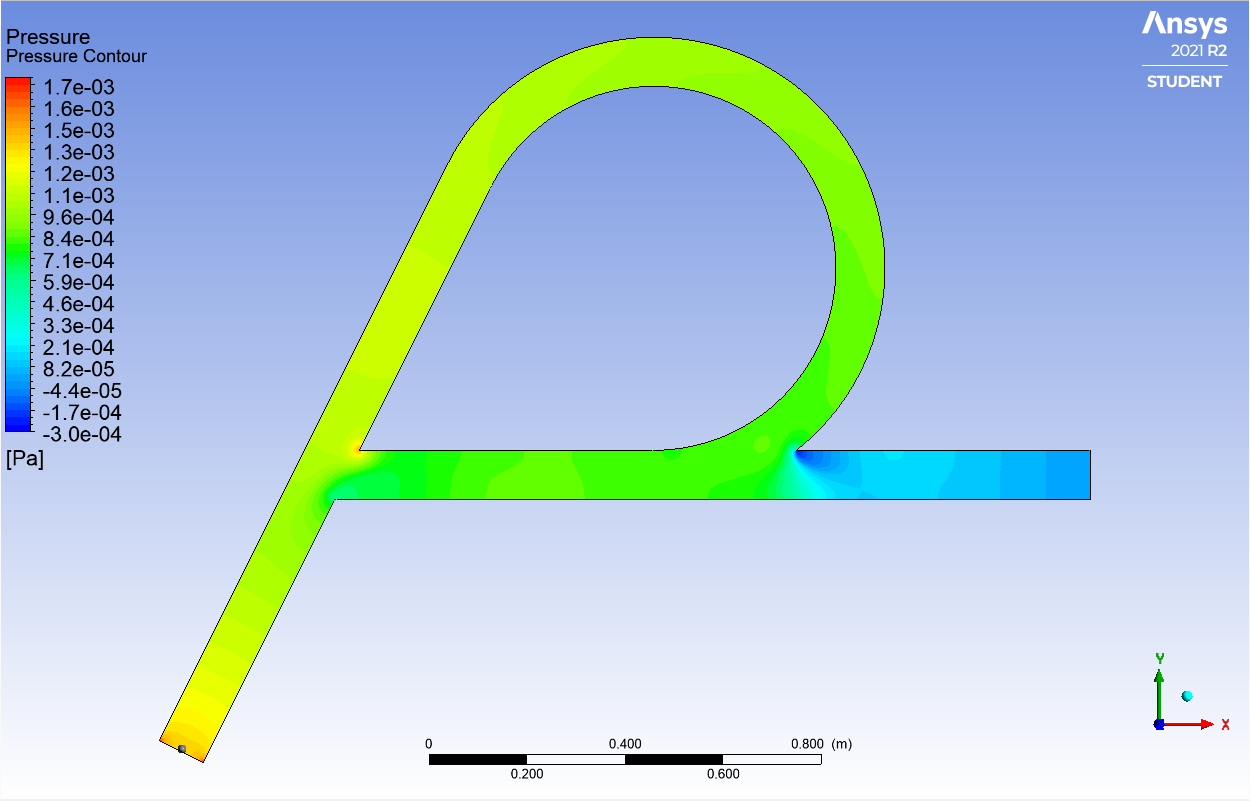
\includegraphics[width=.9\linewidth]{images/task2/L600/reverse181.png}
  \caption{Reverse flow with Re = 181}
  \label{fig:x_d_norm_actual}
\end{subfigure}
~
\begin{subfigure}{.45\textwidth}
  \centering
  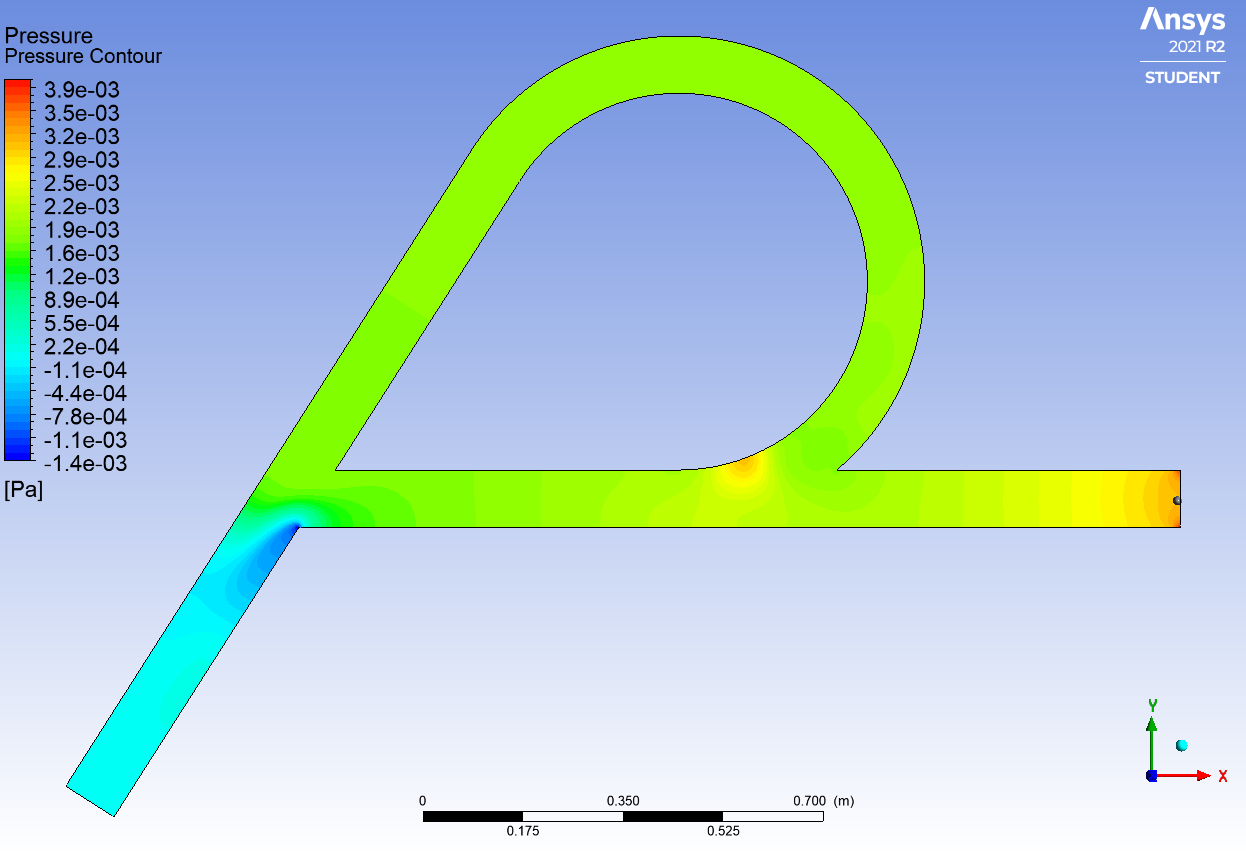
\includegraphics[width=.9\linewidth]{images/task2/L600/forward362.png}
  \caption{Forward flow Re = 362}
  \label{fig:x_d_norm}
\end{subfigure}%
~
\begin{subfigure}{.45\textwidth}
  \centering
  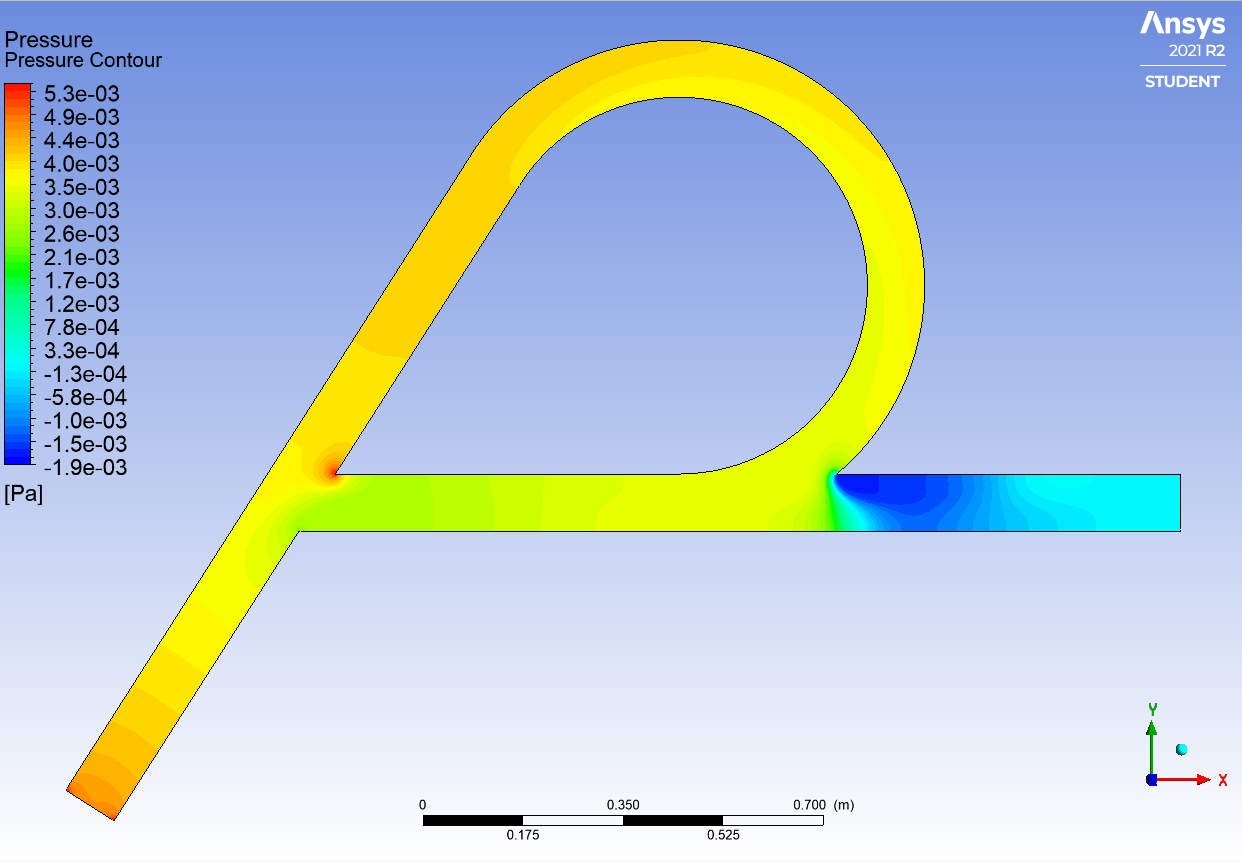
\includegraphics[width=.9\linewidth]{images/task2/L600/reverse362.png}
  \caption{Reverse flow with Re = 362}
  \label{fig:x_d_norm_actual}
\end{subfigure}
~
\begin{subfigure}{.45\textwidth}
  \centering
  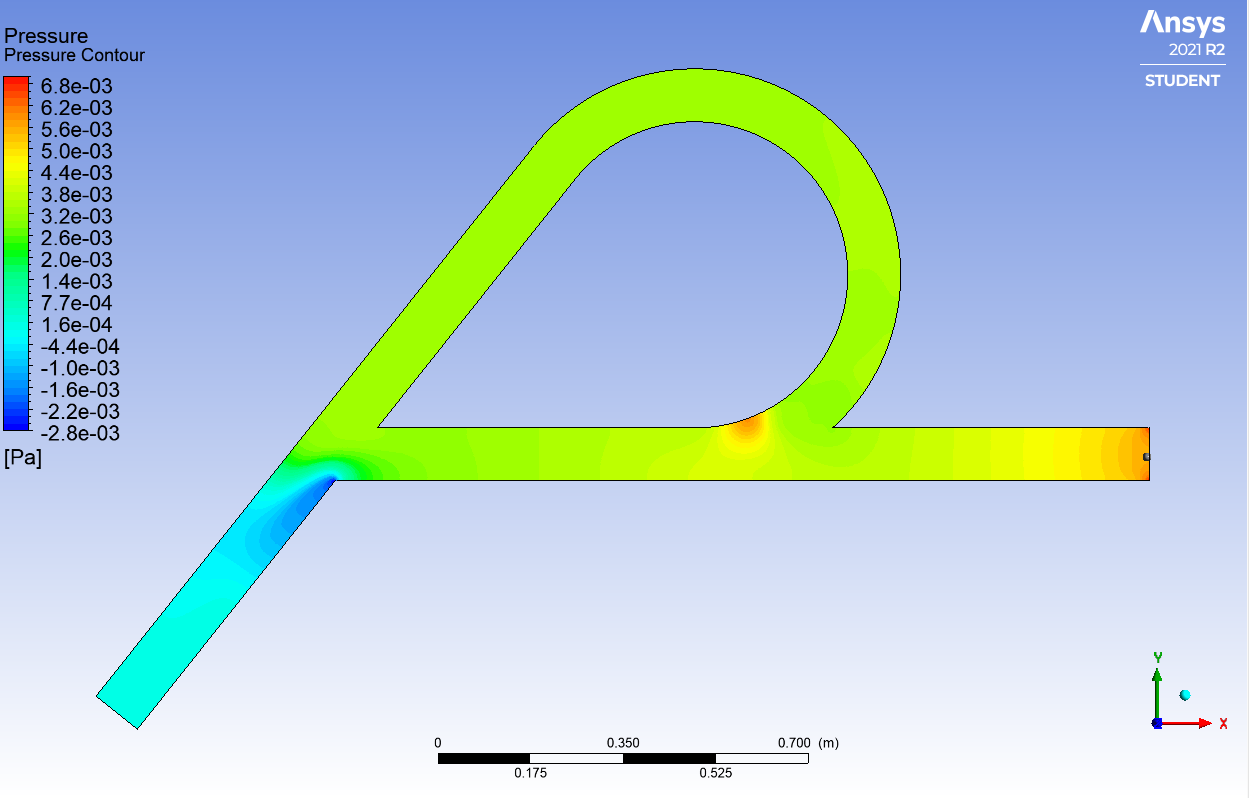
\includegraphics[width=.9\linewidth]{images/task2/L600/forward543.png}
  \caption{Forward flow Re = 543}
  \label{fig:x_d_norm}
\end{subfigure}%
~
\begin{subfigure}{.45\textwidth}
  \centering
  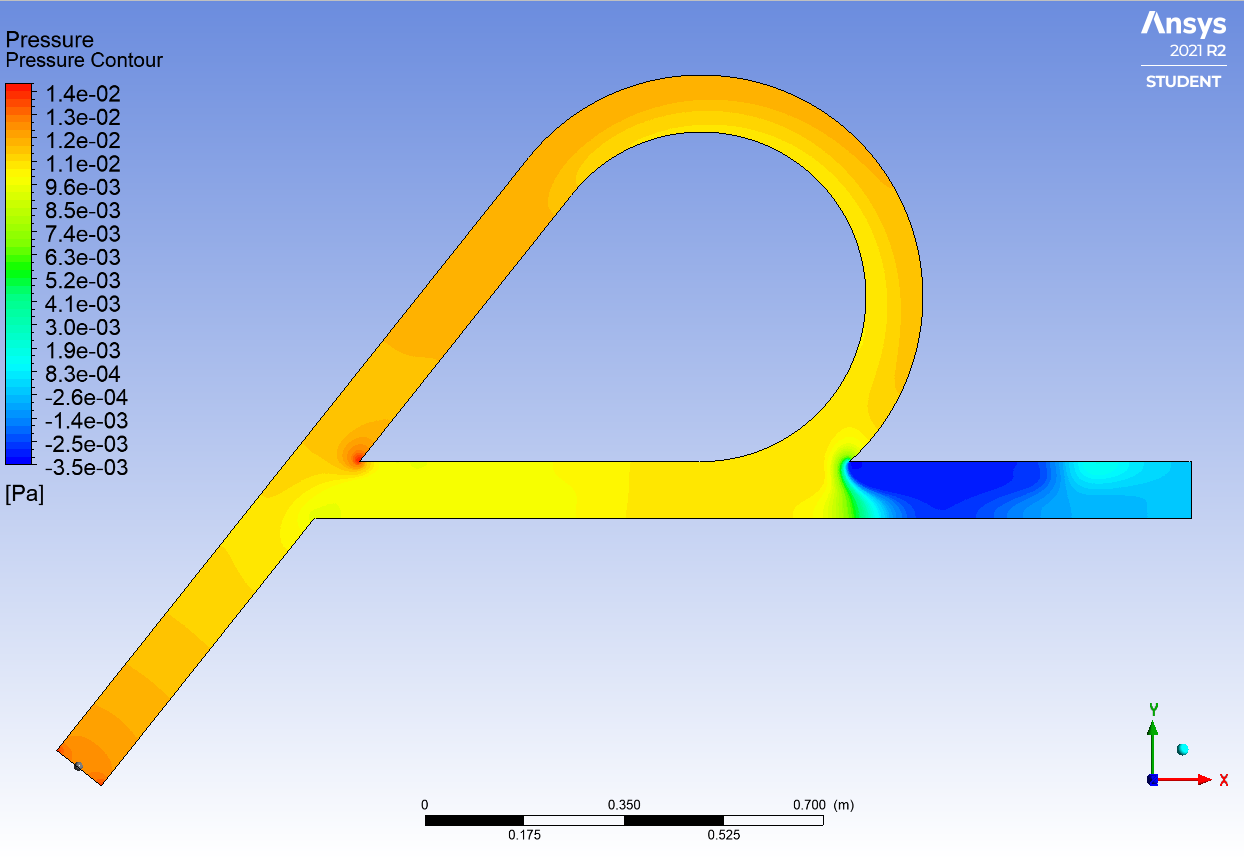
\includegraphics[width=.9\linewidth]{images/task2/L600/reverse543.png}
  \caption{Reverse flow with Re = 543}
  \label{fig:x_d_norm_actual}
\end{subfigure}

\caption{Different Pressure Plots where L = 600mm}
\label{fig:l600}
\end{figure}

\subsubsection{Optimization}

Following these steps, valvular conduit diodicities are plotted versus the straight line segments for all 3 of tested Reynolds numbers. After this, polynomial curves have been fitted to the data in order to find the optimum $L$ values which will be used to relate the optimum $L$ values to Reynolds number. The said plot can be seen on Figure \ref{fig:diodi_vs_L} along with their corresponding fitted polynomial curves. The optimum L values extracted for all 3 Reynolds numbers are found as follows:
\begin{itemize}
    \item Re = 181 : $L_{opt} = 450$
    \item Re = 362 : $L_{opt} = 325$
    \item Re = 543 : $L_{opt} = 200$
\end{itemize}

\begin{figure}[H]
    \centering
    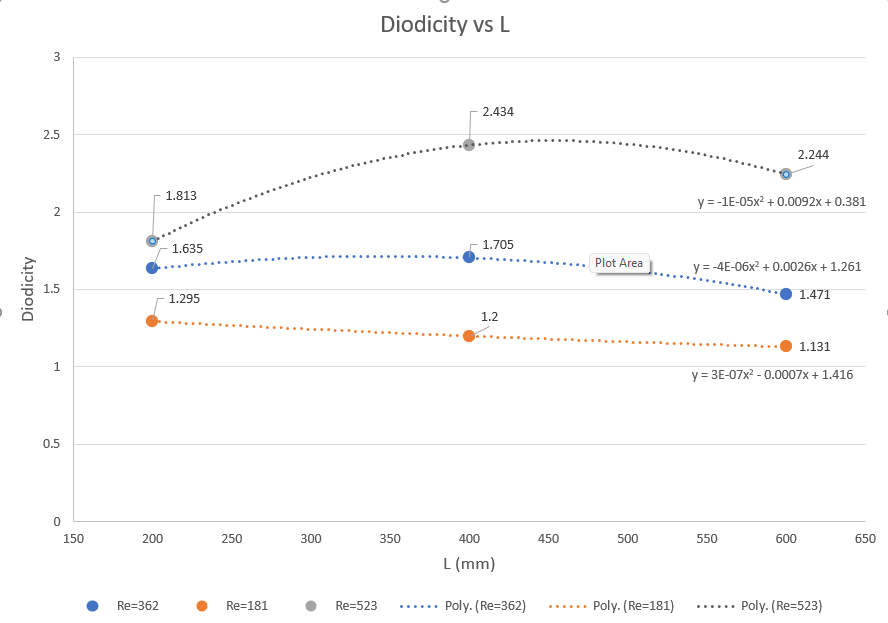
\includegraphics[width = .96\textwidth]{images/task2/diodicity_vs_L_fits.png}
    \caption{Diodicities vs $L$ with plotted curve fits.}
    \label{fig:diodi_vs_L}
\end{figure}


Now that we have the $L_{opt} values$ for 3 different Reynolds numbers, the next step is to try and relate these two and fit a curve accordingly. Figure \ref{fig:LWvsRe} shows this relation along with the equation for the fitted curve. 


\begin{figure}[H]
    \centering
    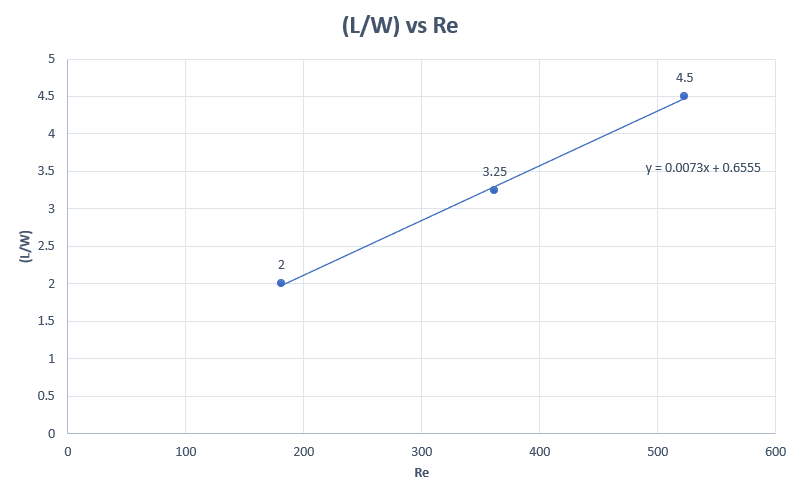
\includegraphics[width = .96\textwidth]{images/task2/LW_vs_Re.png}
    \caption{$(L/W)_{opt} vs Re$}
    \label{fig:LWvsRe}
\end{figure}


It can be clearly seen that the data has shown a linear trend with Reynolds number, the necessary ratio getting greater as Re increases. The fitted relation is as follows:

\begin{equation}
    (L/W)_{opt} = 0.65 + 0.007 * Re
\end{equation}

When compared with Truong's solution \cite{truong}, it can be clearly seen that the equations agree, having the same slope and very little error in constant value. For comparison Truong's solution is found as below:
\begin{equation}
    (L/W)_{opt} = 0.58 + 0.007 * Re
\end{equation}


Following these steps, to observe more about this optimization, a new simulation is conducted using Re = 724 and all the optimal parameters available, including the optimized $L$ value found using our own fitted curve. For Re = 724, $L$ is found to be 571.8mm and $\alpha_{opt}$ is found to be $45.408^\circ$. The pressure plots and velocity plots for both directions are shown on Figure \ref{fig:opt}. This configuration resulted in a \textbf{diodicity of 2.89 which is the maximum diodicity found yet.} \\

Besides this maximum diodicity, the pressure plots and velocities are to be discussed. As can be seen clearly, in forward flow, the velocity of the fluid inside the curved section is very low, almost a stable configuration. This allows the curve to interfere significantly less than otherwise. Mainly due to this, we see the less pressure dropped flow in that direction. However, when we examine the same geometry's reverse flow, we see a quite different situation. The fluid is very fast in that section with when united with the straight flow, causes disturbances and results in a very high pressure drop. \\

%%%%%%%%%opt figure %%%%%%%%%%%%%%
\begin{figure}[H]
 \centering
\begin{subfigure}{.45\textwidth}
  \centering
  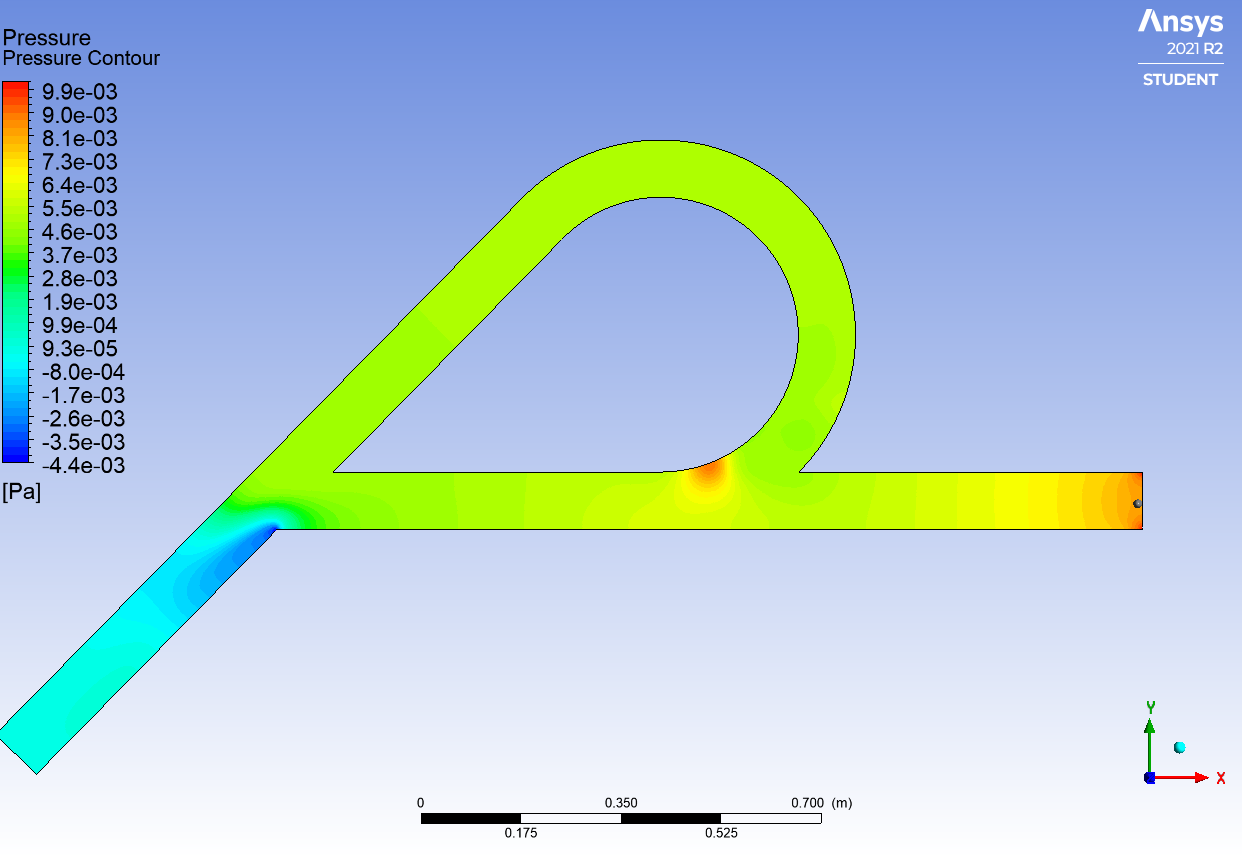
\includegraphics[width=.9\linewidth]{images/task2/myopt/forward_pressure.png}
  \caption{Pressure Plot for Forward Flow}
  \label{fig:x_d_norm}
\end{subfigure}%
~
\begin{subfigure}{.45\textwidth}
  \centering
  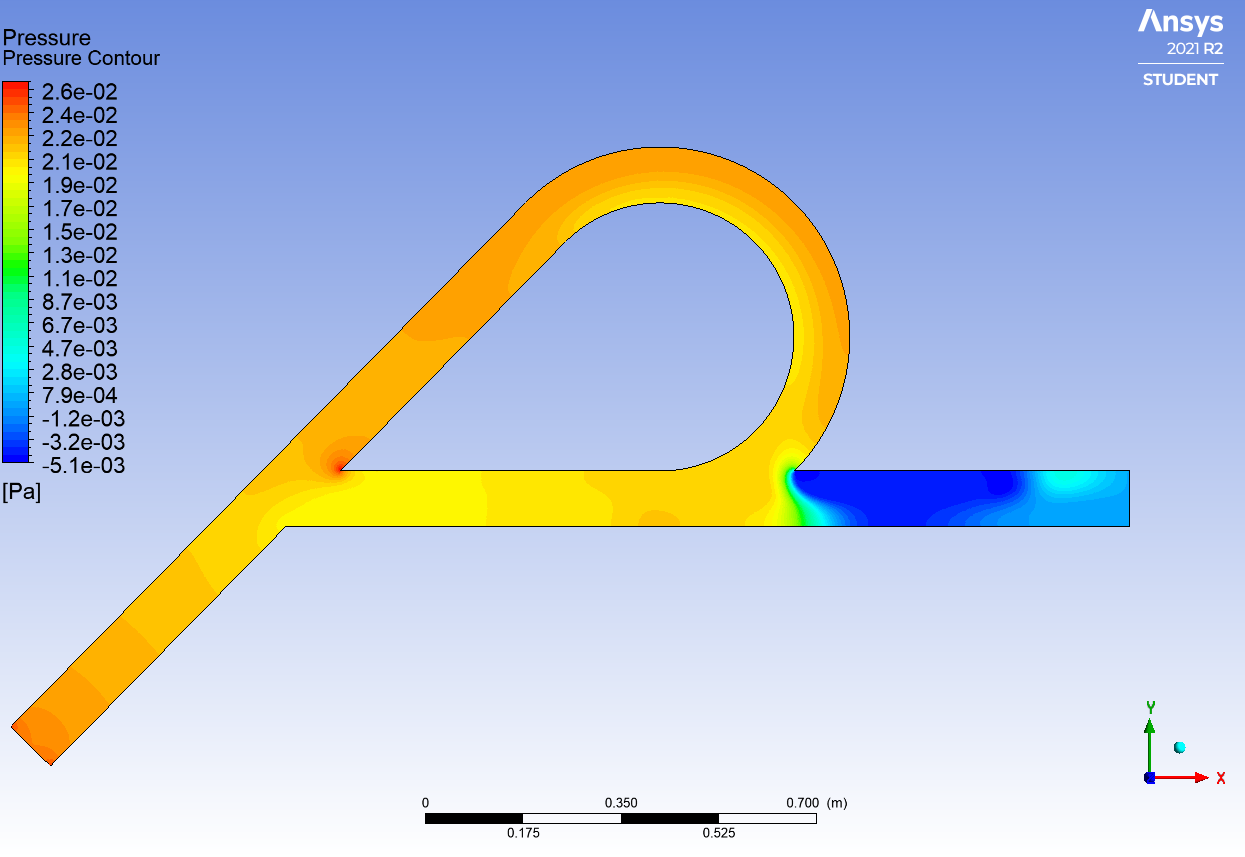
\includegraphics[width=.9\linewidth]{images/task2/myopt/reverse_pressure.png}
  \caption{Pressure Plot for Reverse Flow}
  \label{fig:x_d_norm_actual}
\end{subfigure}
~
\begin{subfigure}{.45\textwidth}
  \centering
  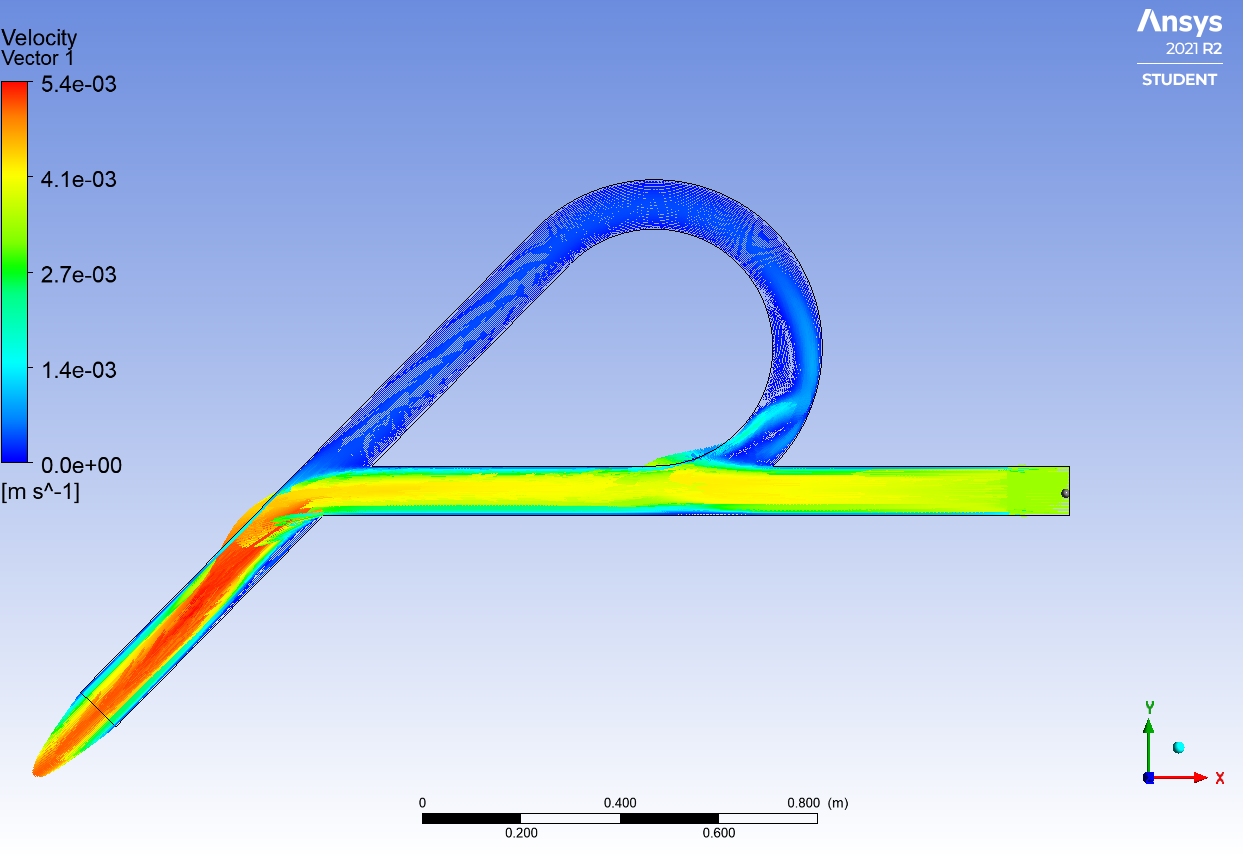
\includegraphics[width=.9\linewidth]{images/task2/myopt/forward_velocity.png}
  \caption{Velocity Plot for Forward Flow}
  \label{fig:x_d_norm}
\end{subfigure}%
~
\begin{subfigure}{.45\textwidth}
  \centering
  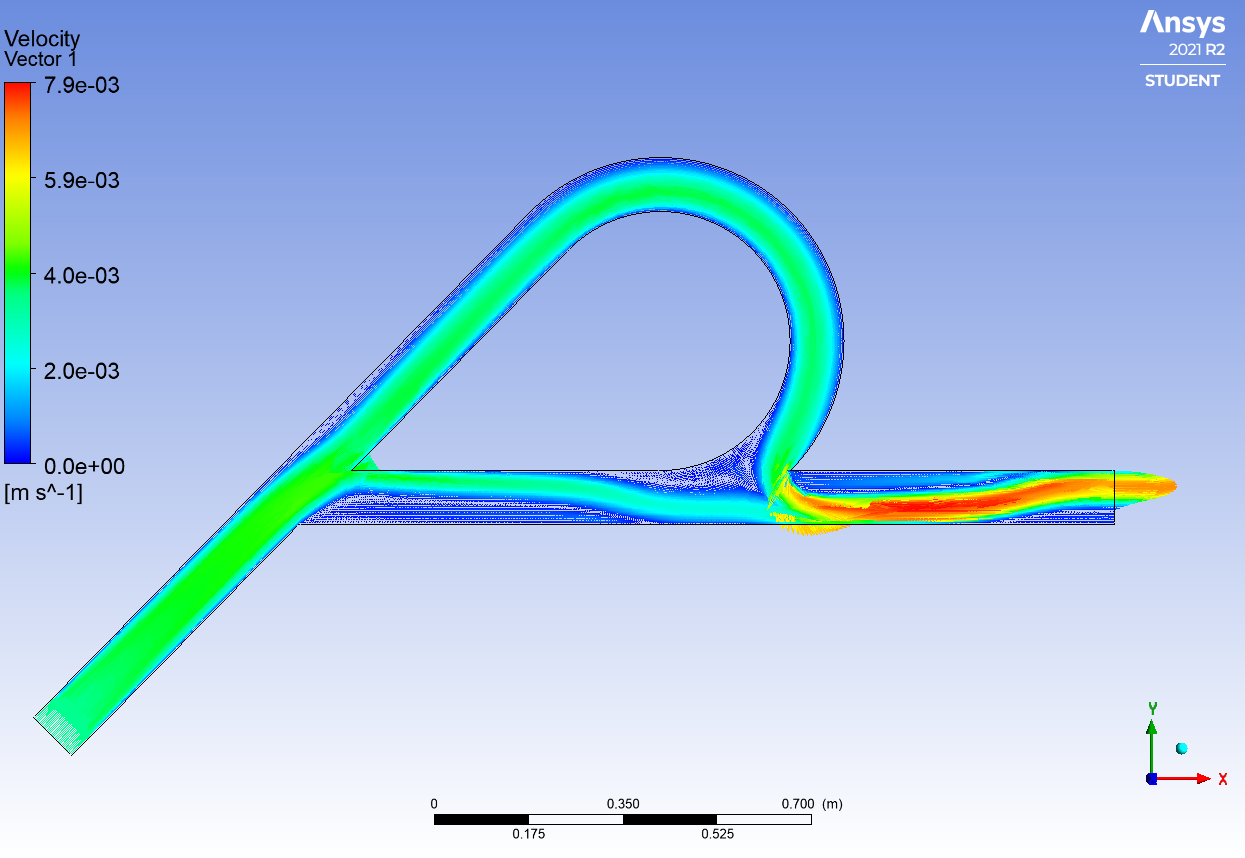
\includegraphics[width=.9\linewidth]{images/task2/myopt/reverse_velocity.png}
  \caption{Velocity Plot for Reverse Flow}
  \label{fig:x_d_norm_actual}
\end{subfigure}

\caption{Optimal L Cases for Re = 724}
\label{fig:opt}
\end{figure}

These comments can also be supported by examining the pressure plots. The pressure plot for reverse flow shows that when high pressured 2 flows are collided at the beginning of the $L_2$ segment, the remaining pressure is dropped highly whereas in the forward flow, they collide in a smoother manner which causes less perturbations, therefore less drop in pressure.

